\apendice{Abordagens precursoras de modelagem procedural}
\label{ap:abordagens_precursoras}

Neste apêndice, de maneira cronológica, serão apresentadas algumas das principais técnicas precursoras de modelagem procedural, tais como \gls{L-Systems} (Seção \ref{sec:l_systems}), \textit{Shape grammars} (Seção \ref{sec:shape_grammars}) e \textit{Split grammars} (Seção \ref{sec:split_grammar}).

\section{L-Systems}
\label{sec:l_systems}

Os \gls{L-Systems} foram introduzidos por \citeonline{lindenmayer1968} para referenciar o estudo matemático da estrutura e desenvolvimento de organismos filamentosos. Sua ideia principal consiste em alterar partes de um objeto inicial, aplicando sucessivas regras de substituição, com objetivo de gerar objetos mais elaborados.

Conforme descrito por \citeonline{simon2011}, uma forma é processada em duas etapas separadas. Na primeira, é realizado um processo de derivação a partir de um elemento inicial, o axioma. Na segunda, a \textit{string} pode ser interpretada geometricamente utilizando gráficos tartaruga. Nos gráficos tartaruga, a interpretação geométrica é obtida tomando cada símbolo como um desenho ou comando de movimento. Sintaticamente, um estado da tartaruga é dado pelo terceto $(x, y, \alpha)$, onde $(x, y)$ representa uma posição cartesiana, e $\alpha$ representa um ângulo que define a direção para qual a tartaruga está voltada. Dados um tamanho de passo $d$ e um ângulo $\beta$, a tartaruga pode responder aos seguintes comandos:

\vspace{0.5cm}

\begin{description}
    \item $F$ \quad Mover à frente uma distância $d$. Desta maneira, o estado da tartaruga muda para $(x', y', \alpha)$, onde $x' = x + d cos(\alpha)$ e $y' = y + d sen(\alpha)$, ou seja, uma linha entre $(x, y)$ e $(x', y')$ é desenhada;
    
    \item $+$ \quad Girar à esquerda por um ângulo $\beta$, fazendo o estado mudar para $(x, y, \alpha + \beta)$;
    
    \item $-$ \quad Girar à direita por um ângulo $\beta$, fazendo o estado mudar para $(x, y, \alpha - \beta)$;
    
    \item $[$ \quad \, Empilhar a posição atual na pilha de localização;
    
    \item $]$ \quad \, Ir para a posição gravada no topo da pilha e a desempilhar.
\end{description}

\vspace{0.5cm}

Historicamente, $F$, $+$, $-$, foram os primeiros símbolos introduzidos visando a modelagem de curvas fractais. Para modelar estruturas ramificadas, como plantas e árvores, os dois símbolos de colchetes foram adicionados, um para registrar a posição atual da tartaruga em uma pilha, e outro para recuperá-la \cite{simon2011}.

O floco de neve de Von Koch, representado na Figura \ref{fig:von_koch_snowflake}, é um exemplo clássico de curva fractal gerado por \gls{L-Systems}. O axioma é $\omega = F ++ F ++ F$, e a gramática é composta por uma única regra $F \rightarrow F - F ++ F - F$. Cada rotação corresponde a um ângulo $\alpha = 60$. A representação geométrica é mostrada para diferentes valores de $n$ \cite{simon2011}, parâmetro que representa a quantidade de iterações da derivação.
	
\begin{figure}[h!]
	\centering
	\captionsetup{width=15cm}
	\Caption{\label{fig:von_koch_snowflake} Geração do floco de neve de Von Koch utilizando \gls{L-Systems}.}	
	\UFCfig{}{
		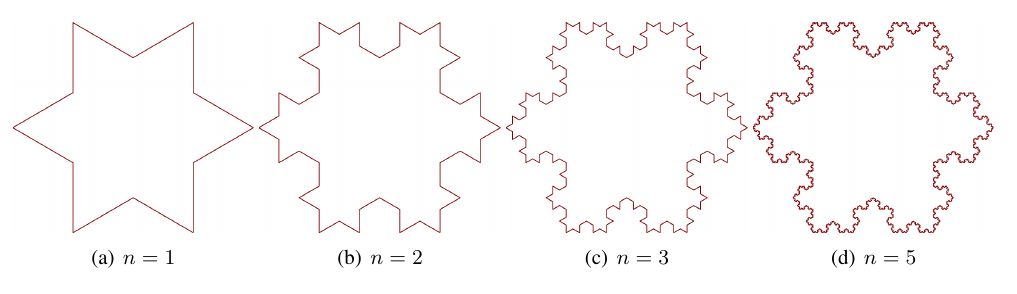
\includegraphics[width=15cm]{figuras/von_koch_snowflake.png}
	}
	{\Fonte{\cite{simon2011}}}	
\end{figure}

A Figura \ref{fig:algae} representa o sistema de uma alga, com intuito de ilustrar o uso dos colchetes. O axioma é $\omega = F$, e uma única regra $F \rightarrow F [+F] F [-F] [F]$ cria duas ramificações. São mostradas diferentes escalas de representação para um ângulo $\alpha = 25.7$ \cite{simon2011}. Da mesma maneira como no exemplo anterior, a representação geométrica é mostrada para diferentes valores de $n$. Além disto, por meio da extensão da gramática e das regras é possível obter resultados similares ao da Figura \ref{fig:l-system3d}.

\begin{figure}[h!]
	\centering
	\captionsetup{width=15cm}
	\Caption{\label{fig:algae} Geração de um modelo de alga utilizando \gls{L-Systems}.}	
	\UFCfig{}{
		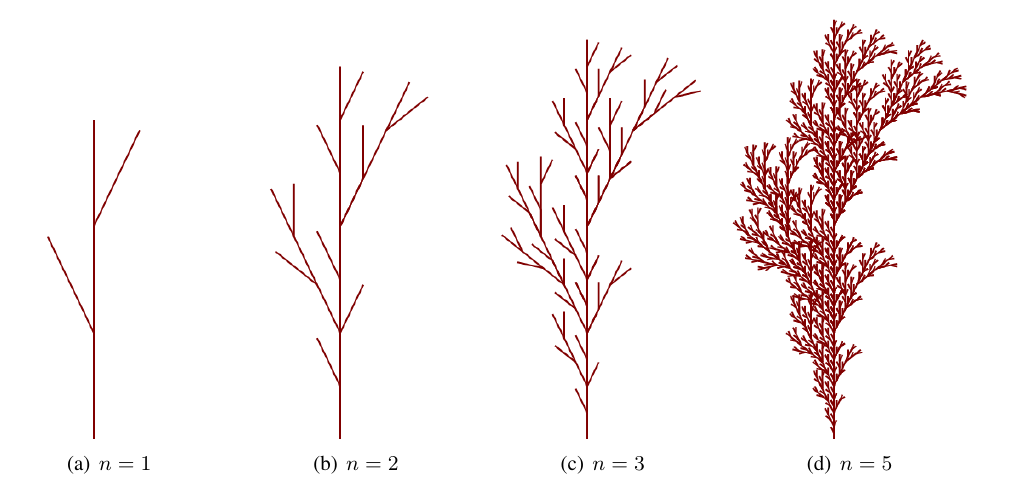
\includegraphics[width=15cm]{figuras/algae.png}
	}
	{\Fonte{\cite{simon2011}}}	
\end{figure}

\begin{figure}[h!]
	\centering
	\captionsetup{width=15cm}
	\Caption{\label{fig:l-system3d} Renderização tridimensional do modelo de uma \textit{Mycelis}.}	
	\UFCfig{}{
		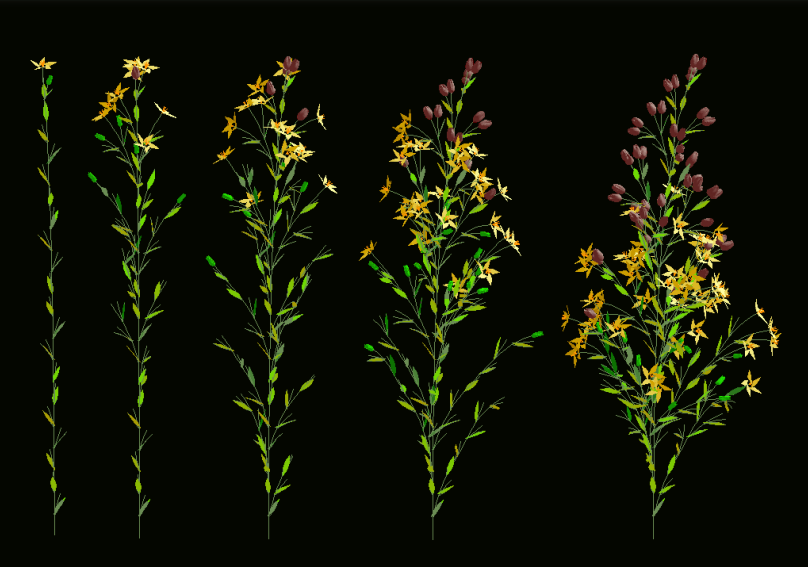
\includegraphics[width=14cm]{figuras/l-systems_plant.png}
	}
	{\Fonte{\cite{lindenmayer1996}}}	
\end{figure}

\section{Shape Grammars}
\label{sec:shape_grammars}

A ideia central das \textit{shape grammars} para criação de modelos 3D é iniciar com uma forma básica, como um cubo, e modificá-lo até que se pareça com o modelo desejado. Este procedimento é realizado aplicando-se várias operações à forma básica, como translação e rotação, até outras mais complexas, como extrusão e divisão, resultando em um modelo mais elaborado. O formalismo das \textit{shape grammars} é dado pela declaração de um estado inicial (axioma), bem como pela atribuição de  símbolos às formas, e também pela definição de regras de produção, que ditam como gerar símbolos e como aplicar as diferentes operações. Uma vez que as operações podem criar novas formas e o modelo resultante depende do encadeamento de múltiplas operações, geralmente, é utilizada uma árvore de derivação para armazenar tal sequência \cite{haubenwallner2016}.

\citeonline{stiny1972} introduziram as \textit{shape grammars} para representar a geração procedural de geometria. Por definição, uma \textit{shape grammar} é uma quádrupla $(V, L, R, \omega)$, onde:

\begin{itemize}
    \item $V$: é um conjunto finito de formas (vocabulário);
    \item $L$: é um conjunto finito de símbolos (rótulos);
    \item $R$: é um conjunto finito de regras no formato $\alpha \rightarrow \beta$, onde $\alpha$ e $\beta$ são formas rotuladas;
    \item $\omega$: é uma forma atômica chamada de axioma.
\end{itemize}

Uma regra $\alpha \rightarrow \beta$ se aplica a uma dada forma $\gamma$ se existe uma transformação $\delta$, tal que $\delta(\alpha)$ está contido em $\gamma$. Após a aplicação de uma regra, a forma de saída é obtida substituindo-se na forma $\gamma$, a subforma $\delta(\alpha)$ por $\delta(\beta)$.

A Figura \ref{fig:greek_church} ilustra um exemplo clássico de \textit{shape grammar}, criado por \citeonline{knight1995}, para descrever a planta de igrejas no formato de cruz grega. Contém uma única regra, transformando um retângulo em outros dois perpendiculares. Na primeira linha, define-se a única regra da gramática. Na segunda linha, apresenta-se uma possível derivação em $n$ etapas, a partir de um retângulo como axioma.

\begin{figure}[h!]
	\centering
	\captionsetup{width=15cm}
	\Caption{\label{fig:greek_church} Gramática para gerar planta de igreja na forma de cruz grega.}	
	\UFCfig{}{
		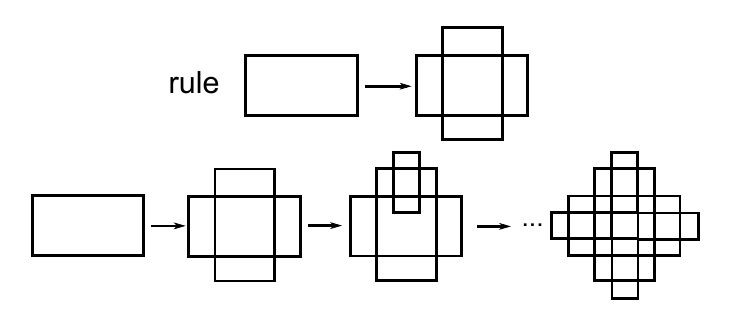
\includegraphics[width=14cm]{figuras/greek_cross_church.png}
	}
	{\Fonte{\cite{knight1995}}}	
\end{figure}


Na Figura \ref{fig:shape_grammars}, através de uma perspectiva cronológica, \citeonline{gu2018} representam os diferentes desenvolvimentos que ampliaram as \textit{shape grammars} básicas, visando atender diferentes necessidades de \textit{design}.

\begin{figure}[h!]
	\centering
	\captionsetup{width=15cm}
	\Caption{\label{fig:shape_grammars} Diagrama que descreve a cronologia das \textit{shape grammars}.}	
	\UFCfig{}{
		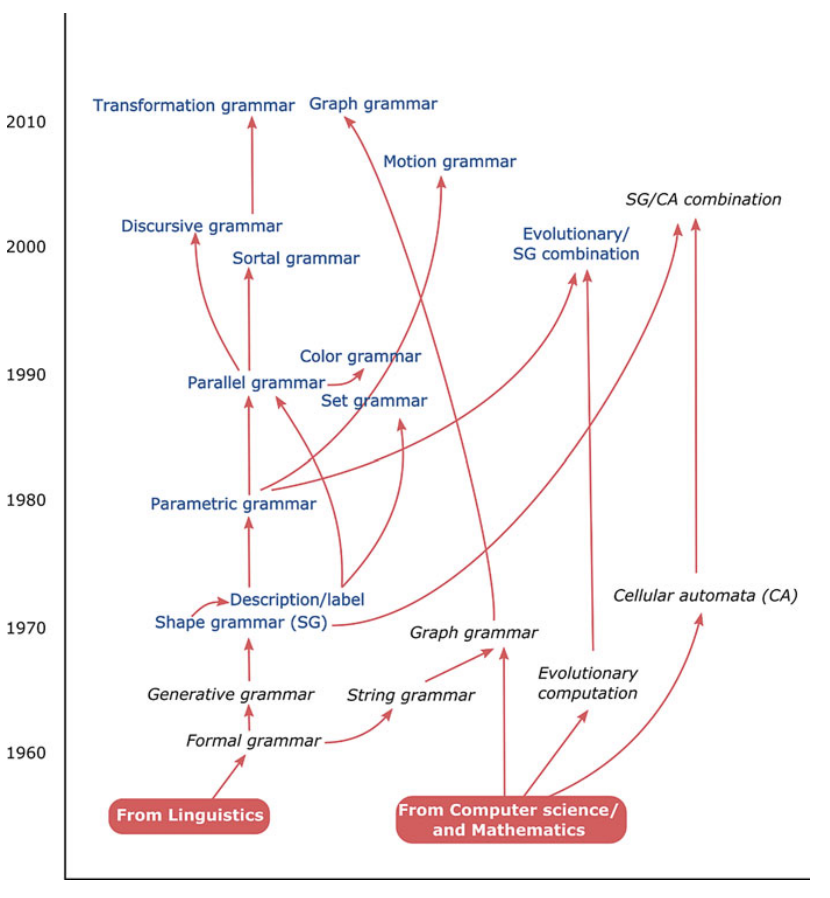
\includegraphics[width=15cm]{figuras/shape_grammars.png}
	}
	{\Fonte{\cite{gu2018}}}	
\end{figure}

\section{Split Grammars}
\label{sec:split_grammar}

As \textit{split grammars} foram introduzidas por \citeonline{wonka2003}, sendo utilizadas, geralmente, para modelagem procedural de fachadas de edifícios. Uma descrição do formalismo é apresentada por \citeonline{francisco2014}, na qual uma \textit{split grammar} é denotada por uma tupla $G = (N, T, \sigma , R)$, onde $N$ representa o conjunto de símbolos não-terminais, $T$ representa o conjunto dos símbolos terminais, $\sigma \in R$ representa a regra inicial, e $R$ representa o conjunto de regras. As regras $r \in R$, por sua vez, têm a forma $LHS \rightarrow RHS$, na qual $LHS \in N$ é um único símbolo não-terminal, e $RHS$ é uma operação \textit{split} que aplicará as regras sucessoras de $LHS$. 

\citeonline{francisco2014} explicam que uma operação de \textit{split} divide uma região geométrica horizontalmente ou verticalmente, e tem a seguinte configuração:

\vspace{0.2cm}

\begin{description}
    \item[] \qquad \qquad $split(axis) \rightarrow (repeat)\{\mu_0 s_0 : r_0, ... , \mu_n s_n : r_n \}$,
\end{description}

\vspace{0.2cm}

\noindent onde \textit{axis} representa o eixo em que a região do espaço será dividida; o símbolo \textit{repeat}, exemplificado na Figura \ref{fig:split_exemplo_2}, é um modificador de regra opcional, que indica se as divisões devem ser aplicadas novamente, caso ainda haja espaço; $s_i$ define o tamanho da divisão a ser aplicada na geometria, que resultará em uma nova região retangular, na qual será aplicada a produção $r_i \in (N \cup T)$; e $\mu_i$ é o modificador da divisão, podendo ser de três tipos:

\textbf{Absoluto:} Utilizado para criar uma nova região de tamanho igual a $s_i$ ao longo do eixo selecionado, se houver espaço suficiente.

\textbf{Aproximado:} Força a nova região a ter tamanho, pelo menos, $s_i$, sendo representado na gramática pelo símbolo $\sim$. Ao final de todas as divisões da operação \textit{split}, se ainda existir espaço sobrando, as regiões marcadas com este modificador aumentarão de tamanho por um número proporcional a $s_i$, fazendo com que toda a região passada como entrada para a regra seja ocupada.

\textbf{Relativo:} Dado um valor $t$ como o tamanho da forma inicial, este modificador, representado na gramática pelo símbolo $'$, atua de maneira a criar uma nova região de tamanho $s_i * t$.

Segundo \citeonline{francisco2014}, numa única operação de \textit{split} é permitido que cada divisão possua um modificador diferente. Na Figura \ref{fig:split_exemplo_1}, por exemplo, é mostrado o uso dos modificadores absoluto e aproximado em uma mesma operação, através da regra $Facade \rightarrow split(Y){4 : GroundFloor, \sim 1 : UpperFloors}$. A Figura \ref{fig:split_exemplo_2}, por sua vez, ilustra o uso do \textit{repeat}, por meio da regra $S \rightarrow repeat split(X){1 : A, 3 : B, 2 : C}$.

\begin{figure}[h!]
	\centering
	\captionsetup{width=15cm}
	\Caption{\label{fig:split_exemplo_1} Exemplo de \textit{split} com o modificador aproximado ($\sim$).}	
	\UFCfig{}{
		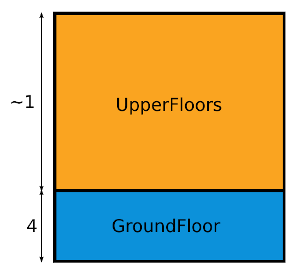
\includegraphics[width=8cm]{figuras/split_exemplo_1.png}
	}
	{\Fonte{\cite{francisco2014}}}	
\end{figure}

\begin{figure}[h!]
	\centering
	\captionsetup{width=15cm}
	\Caption{\label{fig:split_exemplo_2} Exemplo de \textit{split} com repetição.}	
	\UFCfig{}{
		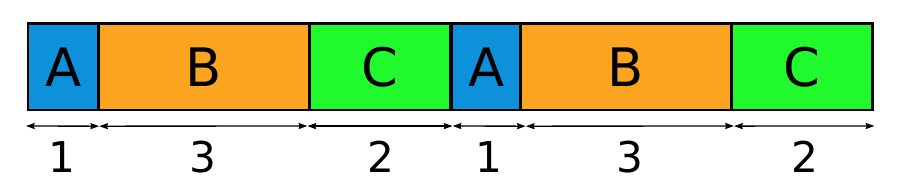
\includegraphics[width=10cm]{figuras/split_exemplo_2.png}
	}
	{\Fonte{\cite{francisco2014}}}	
\end{figure}

Conforme argumentado por \citeonline{francisco2014}, a partir de uma palavra de uma dada gramática, é possível representar uma fachada por meio de uma árvore de derivação, onde cada nó desta árvore associa uma região retangular do espaço a um símbolo da gramática $\varphi \in (T \cup N)$. Os nós intermediários particionam esta região através da aplicação de uma regra $\eta \in R$, e os nós folhas, por sua vez, representam os elementos atômicos que compõem a fachada, como janelas, portas e paredes, os quais são identificados pelos símbolos terminais $\tau \in T$ associados a eles. Para ilustrar esta ideia, a Figura \ref{fig:arvore_derivacao_split} representa a árvore de derivação correspondente à fachada da Figura \ref{fig:fachada_split}.

\begin{figure}[h!]
	\centering
	\captionsetup{width=15cm}
	\Caption{\label{fig:arvore_derivacao_split} Árvore de derivação referente à fachada representada na Figura \ref{fig:fachada_split}.}	
	\UFCfig{}{
		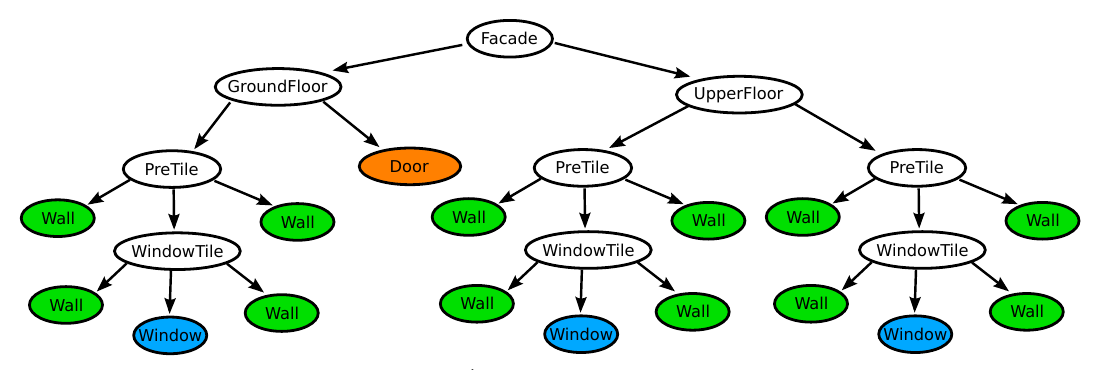
\includegraphics[width=15cm]{figuras/arvore_derivacao_split.png}
	}
	{\Fonte{\cite{francisco2014}}}	
\end{figure}

\begin{figure}[h!]
	\centering
	\captionsetup{width=15cm}
	\Caption{\label{fig:fachada_split} Fachada associada à árvore de derivação da Figura \ref{fig:arvore_derivacao_split}.}	
	\UFCfig{}{
		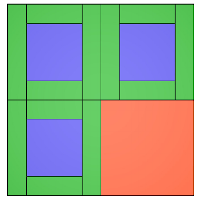
\includegraphics[width=7cm]{figuras/fachada_split.png}
	}
	{\Fonte{\cite{francisco2014}}}	
\end{figure}